\documentclass{beamer}

% {{{ beamer stuffs
\setbeamertemplate{footline}[frame number]
\beamertemplatenavigationsymbolsempty%

\AtBeginSection[]{%
  \begin{frame}<beamer>{Plan}
    \tableofcontents[currentsection]
  \end{frame}
}
\AtBeginSubsection[]{%
  \begin{frame}<beamer>{Plan}
    \tableofcontents[currentsubsection]
  \end{frame}
}
% }}}

\usepackage{fontspec}
\usepackage{hyperref}
\usepackage{pdflscape}

\title{CRAPS Kernel}
\subtitle{Final presentation}
\author{
       Maxime Arthaud
  \and Korantin Auguste
  \and Martin Carton
  \and Étienne Lebrun
}
\titlegraphic{
\includegraphics[width=0.5\textwidth]{fig/LogoEnseeiht.png}}
\date{March 13, 2015}

\begin{document}
  \begin{frame}
    \titlepage%
  \end{frame}

  \section{The project}
    \begin{frame}{Presentation}
      \begin{itemize}
        \item Implement a basic operating system on CRAPS
          \begin{itemize}
            \item CRAPS: processor architecture developed by Jean-Christophe
              Buisson for first year students
          \end{itemize}
        \item Goal: make a operating system course
          \begin{itemize}
            \item based on what student know
            \item adding a continuity in courses
          \end{itemize}
      \end{itemize}
    \end{frame}

    \begin{frame}
      \begin{figure}
        \centering
        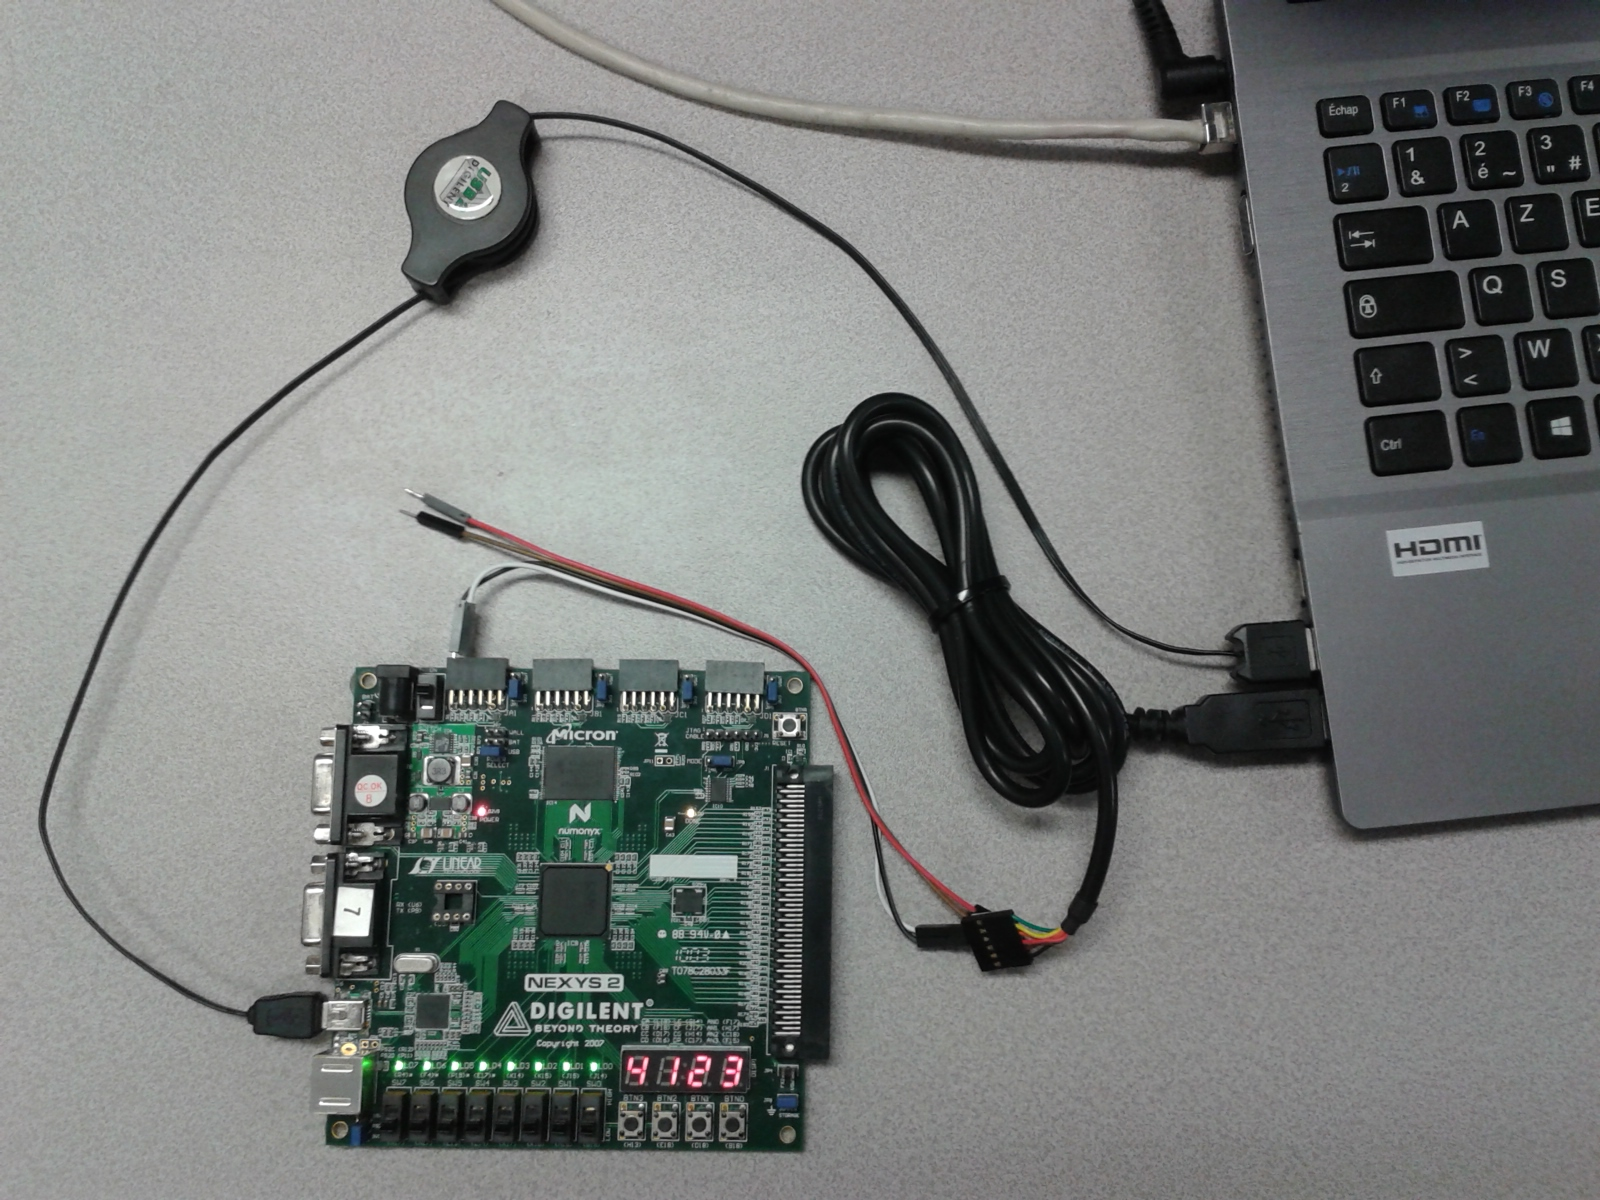
\includegraphics[width=\textwidth, keepaspectratio]{fig/Nexys2.jpg}
        \caption{A Nexys2 board}
      \end{figure}
    \end{frame}

    \begin{frame}{Goal}
      It should show students how a basic operating system works:
        \begin{itemize}
          \item scheduling
          \item interrupts
          \item communications
          \item memory management
        \end{itemize}
    \end{frame}

  \section{Project management}
    \subsection{Team}
      \begin{frame}{Team organization}
        \begin{itemize}
          \item Korantin Auguste as \textit{developer}
          \item Maxime Arthaud as \textit{tester}
          \item Martin Carton as \textit{project leader}
          \item Étienne Lebrun as \textit{quality manager}
        \end{itemize}
      \end{frame}

    \subsection{Project organization}
      \begin{frame}{Risks management}
        We were able to identify real risks, and mitigate them:
        \begin{itemize}
          \item Damaged FPGA
          \item Unable to integrate more RAM
          \item Serial too slow
        \end{itemize}
      \end{frame}

      \begin{frame}{Specifications}
        \begin{itemize}
          \item First week of the project
          \item We identified three main tasks:
            \begin{itemize}
              \item The compiler
              \item The modifications to the processor
              \item The kernel
            \end{itemize}
          \end{itemize}
      \end{frame}

      \begin{frame}{Calendar}
      \end{frame}

      \begin{frame}
        \begin{figure}
          \includegraphics[height=\textheight, width=\textwidth, keepaspectratio]
                          {build/Gantt.pdf}
        \end{figure}
      \end{frame}

  \section{Processor Changes}
    \begin{landscape}
        \begin{frame}
            \includegraphics[scale=0.22]
                            {build/micromachine_updated_fromsvg.pdf}

        \end{frame}
    \end{landscape}

  \section{Implementation}
    \begin{frame}{Compiler}
      \begin{itemize}
        \item Based on the compiler project from the second-year classes.
        \item Language: a (quite large!) subset of C.
        \item Various optimizations.
      \end{itemize}
    \end{frame}

    \begin{frame}{Interrupts}
      \begin{itemize}
        \item Processor modifications.
        \item Priority support.
        \item Interrupt table.
      \end{itemize}
    \end{frame}

    \begin{frame}{Scheduler}
      \begin{itemize}
        \item New interrupt based on the PWM...
        \item that will trigger a context switch.
      \end{itemize}
    \end{frame}

    \begin{frame}{Serial Port}
      \begin{itemize}
        \item New interrupt.
        \item Limitations.
      \end{itemize}
    \end{frame}

    \begin{frame}{Memory Management}
      \begin{itemize}
        \item dynamic allocation
        \item malloc, free, realloc
        \item very simple implementation
        \item we keep the PID in the block headers
      \end{itemize}
    \end{frame}

    \begin{frame}
      \begin{figure}
        \begin{minipage}[c]{0.5\textwidth}
          \caption{Memory layout}
        \end{minipage}\hfill
        \begin{minipage}[c]{0.5\textwidth}
          \includegraphics[height=\textheight]{build/memory_layout_fromsvg.pdf}
        \end{minipage}
      \end{figure}
    \end{frame}

    \subsection{Dynamic loading}
      \begin{frame}
        \begin{itemize}
          \item Not very hard to do\dots
          \item \dots but we had to make the code position-independent.
        \end{itemize}
      \end{frame}

  \section{Final result}
    \begin{frame}{Various processes}
      \begin{itemize}
        \item The shell (most important)
        \item Counter
        \item Leds
        \item \dots and dynamic loading!
      \end{itemize}
    \end{frame}

    \begin{frame}{Demo}
      \begin{itemize}
        \item Compiler
        \item Debugger
        \item Serial console
        \item Process management
      \end{itemize}
    \end{frame}

  \section{Use/Improvements}
    \begin{frame}{Pedagogic use}
        Use in classes? Pedagogic interest.
    \end{frame}
\end{document}
